\documentclass{article}
\usepackage{fancyhdr, graphicx, multicol}

\title{\huge \textbf{Hog Language Reference}}
\author{Jason Halpern\\ Samuel Messing\\ 
        Benjamin Rapaport \\  Kurry Tran \\ Paul Tylkin}

\begin{document}
\maketitle
\newpage

\section{Introduction}
\label{sec:introduction}

As data sets have grown in size, so have the complexities of dealing with them.
For instance, consider wanting to generate counts for all the words in \emph{War
and Peace} by means of distributed computation. Writing in Java and using Hadoop
MapReduce (TM), a simple solution takes over 50 lines of code, as the programmer
is required to specify intermediate objects not directly related to the desired
computation, but required simply to get Hadoop to function properly. Our goal is
to produce a language that can express the same computation in about 10 lines.

\subsection{The MapReduce Framework}
\label{sub:mapreduce}

With the explosion in the size of datasets that companies have had to manage in
recent years there are many new challenges that they face. Many companies and
organizations have to handle the processing of datasets that are terabytes or even
petabytes in size. The first challenge in this large-scale processing is how to
make sense of all this data. More importantly, how can they process and manipulate
the data in a time efficient and reliable manner. The second challenge is how they
handle this across their distributed systems. Writing distributed, fault tolerant
programs requires a high level of expertise and knowledge of parallel systems.

This was an obvious challenge to the company that has to process more data than any
company on earth, Google. In response to this need, a group of engineers at Google
developed their MapReduce framework in 2004. This high-level framework could be
used for of a variety of tasks, including handling search queries, indexing crawled
documents and processing logs. The software framework was developed to handle
computations on massive datasets that are distributed across hundreds or even
thousands of machines. The motivation behind MapReduce was to create a unified
framework that abstracted away many of the low level details from programmers, so
they would not have to be concerned with how the data is distributed, how the
computation is parallelized and how all this is done in a fault tolerant manner.
MapReduce provides fault tolerance in software rather than in hardware. MapReduce
can handle both unstructured data (files) and structured data (databases), but is
predominantly used with files.

The framework partitions the data across different machines, so that the
computations are initially performed on smaller sets of data distributed across the
cluster. Each cluster has a master node that is responsible for coordinating the
efforts among the slave nodes. Each slave node sends periodic heartbeats to the
master node so it can be aware of progress and failure. In the case of failure, the
master node can reassign tasks to other nodes in the cluster. In conjunction with
the underlying MapReduce framework created at Google, the company also had to build
the distributed Google File System (GFS). This file system ``allows programs to
access files efficiently from any computer, so functions can be mapped
everywhere.'' GFS was designed with the same goals as other distributed file
systems, including ``performance, scalability, reliability and availability.''
Another key aspect of the GFS design is fault tolerance and this is achieved by
treating failures as normal and optimizing for ``huge files that are mostly
appended to and then read.''

Within the framework, a programmer is responsible for writing both Map and Reduce
functions. The map function is applied to all of the input data ``in order to
compute a set of intermediate key/value pairs.'' In the map step, the master node
partitions the input data into smaller problems and distributes them across the
worker nodes in the cluster. This step is applied in parallel to all of the input
that has been partitioned across the cluster. Then, the reduce step is responsible
for collecting all the processed data from the slave nodes and formatting the
output. The reduce function is carried out over all the values that have the same
key such that each key has a single value. which is the answer to the problem
MapReduce is trying to solve. The output is done to files in the distributed file
system.

The use of ``a functional model with user-specified map and reduce operations allows (Google) to parallelize large computations
easily and to use re-execution as the primary mechanism for fault tolerance.'' A programmer only has to specify the functions
described above and the system handles the rest of the details. Figure \ref{fig:map_reduce_overview} illustrates the execution
flow of a MapReduce program.

\begin{center}
\begin{figure}
  \label{fig:map_reduce_overview}
  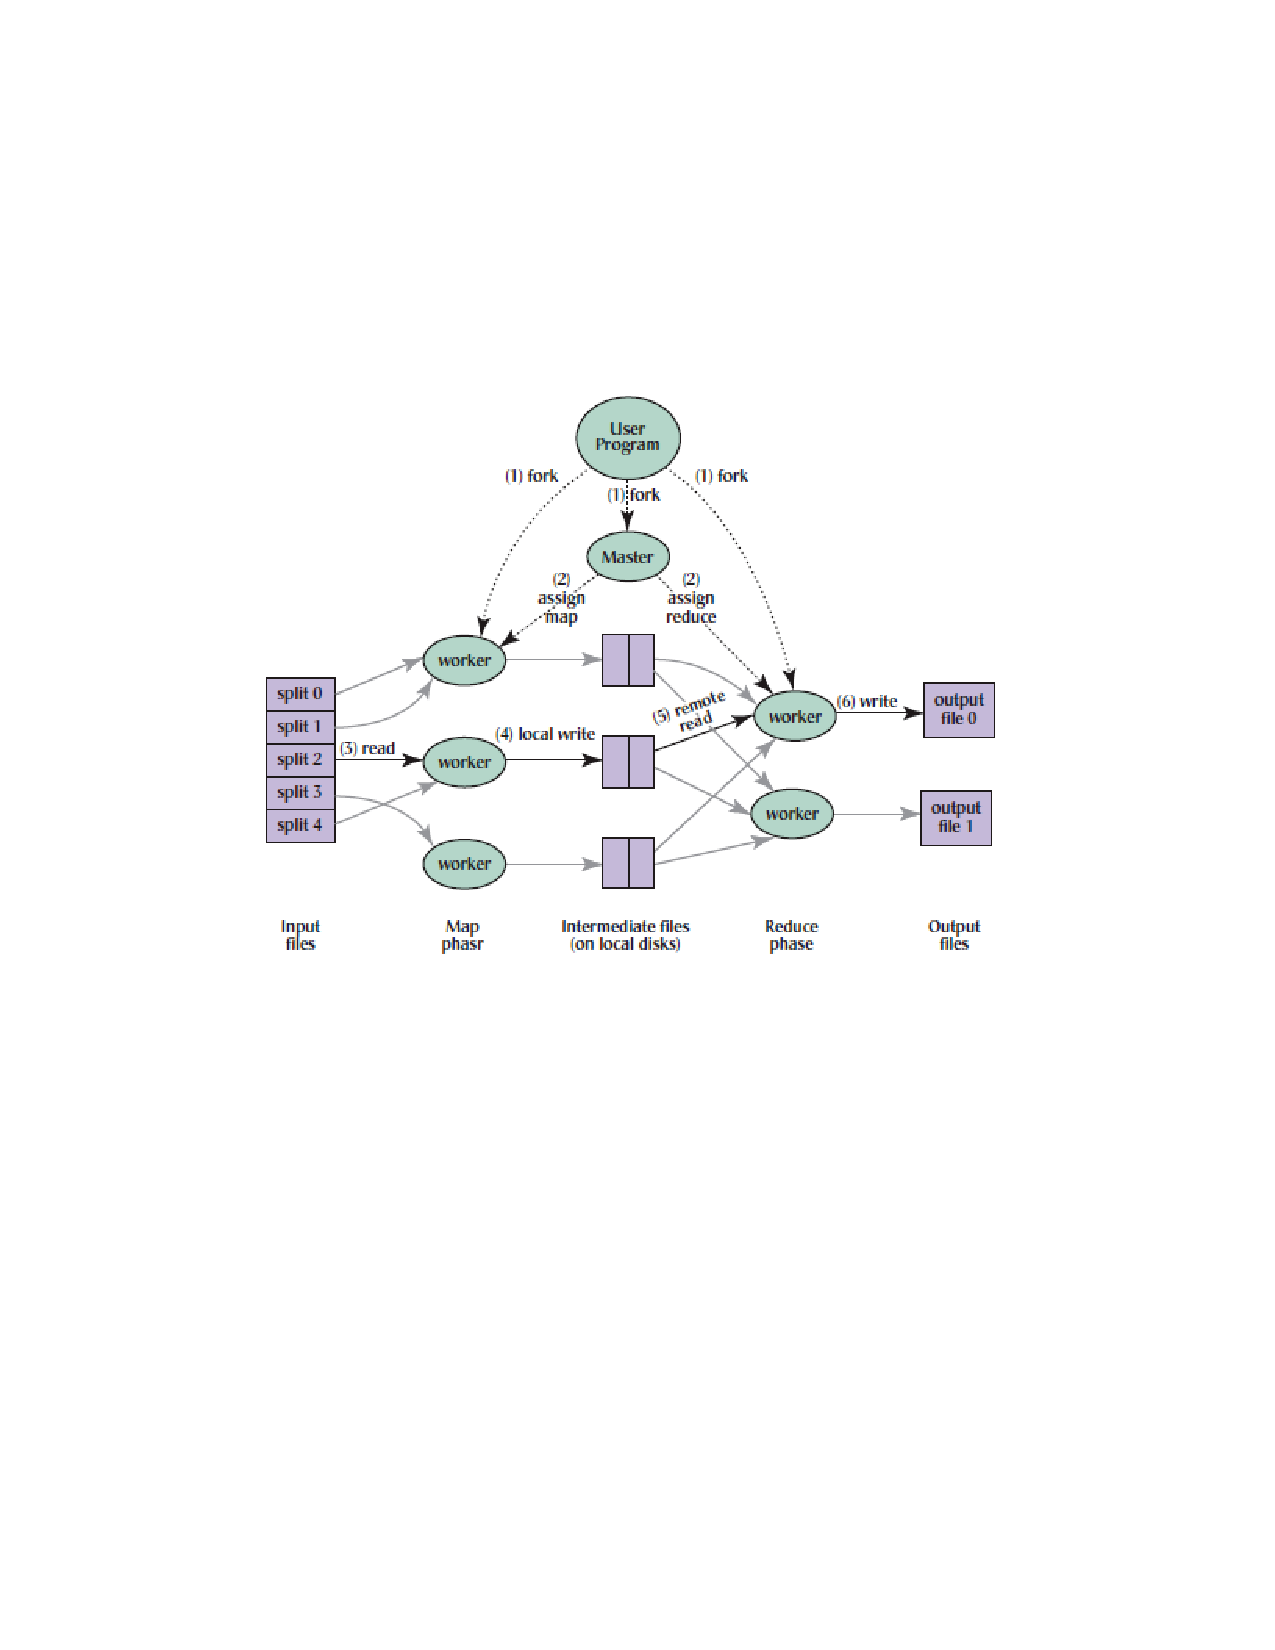
\includegraphics[width=0.85\textwidth]{img/map_reduce_overview.pdf}
  \caption{Overview of the Map Reduce program}
\end{figure}
\end{center}

\subsection{The Hog Language}
\label{sub:hog_language}

Hog is a \textbf{data-oriented}, \textbf{high-level}, scripting language for
creating MapReduce programs. Used alongside Hadoop, Hog enables users to
efficiently carry out \textbf{distributed} computation. Hadoop MapReduce is an
open-source framework for carrying out distributed computation, which is especially
useful for working with large data sets. While it is possible to write code to
carry out computations with Hadoop directly, the framework requires users to
specify low-level details that are often irrelevant to their desired goal.

By building a scripting language on top of Hadoop, we aim to simplify the process.
Built around a \textbf{simple} and highly \textbf{readable} syntax, Hog will let
users focus on what computations they want done, and not how they want to do them.
Hog takes care of all the low-level details required to run computations on
Hadoop’s distributed network. All a user needs to do is tell Hog the location of
their valid Hadoop instance, and Hog will do the rest.

We intentionally have restricted the scope of Hog to deal with specific problems. For example, Hog's collection objects can
only contain primitive types (preventing such data structures as lists of lists). Also, Hog only supports reading and writing
plaintext files. While these limitations sacrifice the generality of the language, they promote ease of use.

\subsubsection{Guiding Principles} % (fold)
\label{ssub:guiding_principles}

The guiding principles of Hog are:

\begin{itemize}
  \item Anyone can MapReduce
  \item Brevity over verbosity
  \item Simplicity over complexity
\end{itemize}


% subsubsection guiding_princples (end)

\subsection{The (Ideal) Hog User} % (fold)
\label{sub:the_ideal_hog_user}

Hog was designed with a particular user in mind: one that has already learned the basics of programming in a different
programming language (such as Python or Java), but is inexperienced enough to benefit from a highly structured framework for
writing MapReduce programs. The language was designed with the goal of making learning how to write MapReduce programs as easy
as possible. \textbf{@Paul: flesh out if needed}.

% subsection the_ideal_hog_user (end)

\section{Program Structure} % (fold)
\label{sec:program_structure}

\subsection{Overall Structure} % (fold)
\label{sub:overall_structure}

Every Hog program consists of a single source file with a ‘.hog’ extension. This
source file must contain three sections: \tt @Map\rm, and \tt @Reduce\rm, and
\tt @Main \rm and can also include an optional \tt @Functions \rm section. These
sections must be included in the following order:

\begin{verbatim}
    @Functions {
      .
      .
      .
    }
    @Map <type signature> {
      .
      .
      .
    }
    @Reduce <type signature>
      .
      .
      .
    @Main {
      .
      .
      .
    }
\end{verbatim}

% section overall_structure (end)

\subsection{\tt @Functions\rm} % (fold)
\label{sub:tt_functionsrm}

At the top of every Hog program, the programmer has the option to define functions
in a section called \tt @Functions\rm. Any function defined in this section can be
called from any other section of the program, including \tt @Map\rm, and \tt
@Reduce\rm, and can also be called from other functions defined in the \tt
@Functions \rm section. The section containing the functions begins with the
keyword \tt @Functions \rm on its own line, followed by the function definitions.

Function definitions have the form:

\begin{quotation}
  \tt @Functions \rm \\
  \indent \emph{type functionName(parameterList)} \tt \{ \rm \\
  \indent \indent \emph{expressionList} \\
  \indent \tt \} \rm
\end{quotation}

The return-type can be any valid Hog type. The rules regarding legal function-names
are identical to those regarding legal variable identifiers. Each parameter in the
parameter-list consists of a valid Hog type followed by the name of the parameter,
which must also follow the naming rules for identifiers. Parameters in the
parameter-list are separated by commas. The @Functions section ends when the next
Hog section begins.

A complete example of an @Functions section:

\begin{verbatim}
    @Functions
    int min(int a, int b) {
      if (a < b) {
        return a
      } else {
        return b
      }
    }

    list<int> reverseList(list<int> oldList) {
      list<int> newList()
      for (int i = oldList.len()-1; i >= 0; i--) {
        newList.append(oldList.get(i))
      }
      return newList
    }
\end{verbatim}

Function names can be overloaded as long as the function definitions have different
signatures (i.e. parameter lists different in types and/or length). Additionally,
user-defined functions can make reference to other user-defined functions.

% section tt_functionsrm (end)

\subsection{\tt @Map \rm} % (fold)
\label{sub:tt_map_rm}

The map function in a MapReduce program takes as input key-value pairs, performs
the appropriate calculations and procedures, and emits intermediate key-value pairs
as output. Any given input pair may map to zero, one, or multiple output pairs. The
\tt @map \rm section defines the code for the map function.

The \tt @map \rm header must be followed by the signature of the map function, and
then the body of the map function as follows:

\begin{quotation}
  \tt @map ( \rm \emph{type identifier, type identifier} \tt ) -> ( \rm \emph{type, type} \tt ) \{ \\
  \indent \indent . \\
  \indent \indent . \\
  \indent \indent . \\
  \indent \tt \} \rm
\end{quotation}

The first \tt type identifier \rm defines the \emph{\textbf{key}} and the second defines the \emph{\textbf{value}} of the input
key-value pair to the \tt @map \rm function. The identifiers specified for the key and value can be made reference to later
within the \tt @map \rm block. The \tt @map \rm signature is followed by an arrow and another key-value pair, defining the
types of the output of the map function. Notice that identifiers are not specified for the output key and value (said to be
\emph{unnamed}), as these pairs are only produced at the end of the map function. Also note that any code written in the same
scope after an \tt emit() \rm call will be \textbf{\emph{unreachable}}, and will cause a compile-time \tt
UnreachableCodeException\rm.

The map function can include any number of calls to \tt emit()\rm, which outputs
the resulting intermediate key-value pairs for use by the function defined in the
\tt @reduce \rm section. The types of the values passed to the \tt emit() \rm
function must agree with the signature of the output key-value pair as defined in
the \tt @map \rm type signature. All output pairs from the map function are
subsequently grouped by key by the framework, and passed as input to the \tt
@reduce \rm function.

Currently, the only configuration available is for a file to be passed into the map
function one line at a time, with the line of text being the value, and the
corresponding line number as the key. This requires that the input key/value pair
to the map function is of type \tt (int key‐name,text value‐name)\rm. Extending
this to allow for other input formats is a future goal of the Hog language.

The following is an example of a complete \tt @Map \rm section for a program that
counts the number of times each word appears in a set of files. The map function
receives a single line of text, and for each word in the line (as delineated by
whitespace), it emits the word as the key with a value of one. By emitting the word
as the key, we can allow the framework to group by the word, thus calling the
reduce function for every word.

% section tt_map_rm (end)

\subsection{\tt @Reduce \rm} % (fold)
\label{sub:tt_reduce_rm}

The reduce function in a MapReduce program takes a list of values that share the
same key, as emitted by the map function, and outputs a smaller set of values to be
associated with another key. The input and output keys do not have to match, though
they often do.

The setup for the reduce section is similar to the map section. However, the input
value for any reduce function is always an iterator over the list of values
associated with its key. The type of the key must be the same as the type of the
key emitted by the map function. The iterator must be an iterator over the type of
the values emitted by the map function.

\begin{quotation}
  \tt @reduce ( \rm \emph{type identifier, type identifier} \tt ) -> ( \rm \emph{type, type} \tt ) \{ \\
  \indent \indent . \\
  \indent \indent . \\
  \indent \indent . \\
  \indent \tt \} \rm
\end{quotation}

As with the map function, the reduce function can emit as many key/value pairs as
the user would like. Any key/value pair emitted by the reduce function is recorded
in the output file.

Below is a sample at \tt @Reduce \rm section, which continues the word count
example, and follows the @mapsample introduce in the previous section.

% subsection tt_reduce_rm (end)

\subsection{\tt @Main \rm} % (fold)
\label{sec:tt_main_rm}

\textbf{@BEN: Fill this in!} Hog.mapReduce()

% subsection tt_main_rm (end)

% section program_structure (end)

\section{Lexical Conventions} % (fold)
\label{sec:lexical_conventions}

\subsection{Tokens} % (fold)
\label{sub:tokens}

\textbf The classes of tokens include the following: identifiers, keywords, constants, string literals, operators and separators. Blanks, tabs, newlines and comments are ignored. If the input is separated into tokens up to a given character, the next token is the longest string of characters that could represent a token.

% subsection tokens (end)

\subsection{Comments} % (fold)
\label{sub:comments}

Multi-line comments are identified by the enclosing character sequences \tt \#\{ \rm and \tt \}\#\rm. Anything within these
enclosing characters is considered a comment, and is completely ignored by the compiler. For example,

\begin{verbatim}
    int i = 0
    #{ these are block
        comments and are ignored
         by the compiler }#
    i++
\end{verbatim}

In the above example, the text \tt these are block comments \textbackslash n comments and are ignored \textbackslash n by the
complier \rm are completely ignored during compilation. Compilation goes directly from the line \tt int i = 0 \rm to the line
\tt i++\rm.

Single-line comments are defined to be strings of text included between a '\tt
\#\rm' symbol on the left-hand side an a newline character ('\tt\textbackslash
n\rm') on the right-hand side.

% subsection comments (end)

\subsection{Identifiers} % (fold)
\label{sub:identifiers}
A valid identifier consists of sequence on contiguous leters, digits, or
underscores. The first character of an identifier must not be a digit.
The identifiers are case sensitive so foo is not the same identifier as Foo. 

\textbf{@kurry: explain what a valid identifier is}

% section identifiers (end)

\subsection{Keywords} % (fold)
\label{sub:keywords}

The reserved words of Hog are a superset of the reserved words of Java, since
Hadoop scripts compile into runnable Java code. The following words are reserved
for use as keywords, and may not be redefined by a programmer:

\begin{multicols}{4}
\tt
\begin{itemize}
  \item[] bool
  \item[] case
  \item[] catch
  \item[] default
  \item[] dict
  \item[] else
  \item[] elseif
  \item[] emit
  \item[] final
  \item[] for
  \item[] foreach
  \item[] hadoop
  \item[] if
  \item[] instanceof
  \item[] int
  \item[] iter
  \item[] list
  \item[] map
  \item[] real
  \item[] return
  \item[] switch
  \item[] text
  \item[] try
  \item[] void
  \item[] while
\end{itemize}
\rm
\end{multicols}

The experienced programmer may note that several of Java's reserved words are missing from this list. Because Hog programs
compile into Java programs, at first blush it would seem that there is the potential here to create invalid java programs. The
Hog compiler is smart enough to recognize when a user uses a Java reserved word as an identifier, and automatically prepends
the text "hog" to avoid any collisions.

% subsection keywords (end)

\subsection{Constants} % (fold)
\label{sub:constants}

\textbf{@Paul: flesh this out}

% subsection constants (end)

\subsection{String Literals} % (fold)
\label{sub:string_literals}
A string literal consists of a sequence of zero of more contiguous characters enclosed
in double quotes, such as "hello". A string literal can also contain escape characters
such as slash-n for the new line character or slash-t for the tab character. 

\textbf{@Kurry: flesh this out as k\&r would}

% subsection string_literals (end)

\subsection{Variable Scope} % (fold)
\label{sub:variable_scope}

Hog implements what is generally referred to as lexical scoping or block scope. An
identifier is valid within its enclosing block. The identifier is also value for
any block nested within its enclosing block.

% subsection variable_scope (end)

% section lexical_conventions (end)

\section{Syntax Notation} % (fold)
\label{sec:syntax_notation}

\textbf In the syntax notation used throughout the Hog manual, different syntactic categories are noted by italic type, and literal words and characters are in typewriter style. 

% sec syntax_notation (end)

\section{Types} % (fold)
\label{sec:types}

\subsection{Basic Types} % (fold)
\label{sub:basic_types}

The basic types of Hog include \tt int \rm (integer numbers, 64 bytes in size), \tt
real \rm (floating point numbers, 64 bytes in size), \tt bool \rm(boolean values,
true or false) and \tt text \rm (Strings, variable in size). Unlike most languages,
Hog includes no basic character type. Instead, a programmer makes use of \tt
text\rm s of size 1.

\emph{Implementation details} Hog’s primitive types are not so primitive. They are
in fact wrappers around Hadoop classes. For instance, Hog’s \tt int \rm type is a
wrapper around Hadoop's \tt IntWritableclass\rm. The following lists for every
primitive type in Hog the corresponding Hadoop class that the type is built on top
of:

\begin{center}
\begin{tabular}{|c|c|}
    \hline
\textbf{Hog Type} & \textbf{Enclosed Hadoop Class} \\ \hline
\tt int & \tt IntWritable \\ \hline
\tt real & \tt DoubleWritable \\ \hline
\t bool & \tt BooleanWrtiable \\ \hline
\tt text & \tt text\textbf{???}\rm \\ \hline
\end{tabular}
\end{center}

% subsection basic_types (end)

\subsection{Derived Types (Collections)} % (fold)
\label{sub:derived_types_collections_}

Derived types include \tt list<T>\rm, \tt set<t>\rm, \tt multiset<t>\rm, and \tt
iter<t>\rm. The \tt list<T> \rm type is an ordered collection of objects of the
same type. The \tt set<T> \rm is an unordered collection of unique objects of the
same type. The \tt multiset<T> \rm is an unordered collection of objects of the
same type, with duplicates allowed. The \tt dict<K,V> \rm is a collection of
key­value pairs, where keys are all of the same type, and values are all of the
same type (keys and values can be of different types from one another). The only
types currently allowed within collections are primitive types, preventing such
constructs as a list of lists. All collections allow for null
entries.\footnote{Note that for \tt set<T>\rm, only one \tt null \rm entry is
allowed, and for \tt map<K,V>\rm, only one \tt null \rm key is allowed.}

% subsection derived_types_collections_ (end)

\subsection{Conversions} % (fold)
\label{sub:conversions}

\textbf{@Paul}

% subsection conversions (end)

% section types (end)

\section{Expressions} % (fold)
\label{sec:expressions}

\subsection{Operators} % (fold)
\label{sub:operators}

\subsubsection{Arithmetic Operators} % (fold)
\label{ssub:arithmetic_operators}

Hog implements all of the standard arithmetic operators. All arithmetic operators are only defined for use between variables of
numeric type (\tt int\rm, \tt real\rm) with the exception that the \tt + \rm operator is also defined for use between two \tt
text \rm variables. In such instances, \tt + \rm is defined as concatenation. Thus, in the following,

\begin{verbatim}
    text face = "face"
    text book = "book"
    text facebook = face + book
\end{verbatim}

After execution, the variable \tt facebook \rm will have the value ``facebook''. No other arithmetic operators are defined for
use with \tt text \rm variables, and \tt + \rm is only valid if both variables are of type \tt text \rm. Otherwise, the program
will result in a compile-time \tt TypeMismatchException\rm. 

When an arithmetic operator is used between two numeric variables of different type, as in,

\begin{verbatim}
    int a = 1
    real b = 2.0
    a + b
\end{verbatim}

the non-\tt real\rm variable will be \textbf{\emph{coerced}} into a \tt real \rm before the evaluation of the statement, so
that both operands have the same type. Therefore, the resulting type of the value of an expression involving an arithmetic
operator and one or two operand of type \tt real \rm is always \tt real\rm.

If one of the operands happens to have a \tt null \rm value (for instance, if a variable is \textbf{\emph{uninitialized}}),
then the resulting operation will cause a run-time \tt NullValueException\rm, and the program will crash.

\begin{center}
\begin{tabular}{|c|c|c|c|c|}

\hline \textbf{Operator} & \textbf{Arity} & \textbf{Associativity} &
\textbf{Precedence Level} & \textbf{Behavior} \\ \hline
\tt + \rm & binary & left & 0 & addition \\ \hline
\tt - \rm & binary & left & 0 & minus \\ \hline
\tt * \rm & binary & left & 1 & multiplication \\ \hline
\tt / \rm & binary & left & 1 & division \\ \hline
\tt \% \rm & binary & left & 2 \textbf{??} & mod\footnote{Follows Java's 
\tt \% \rm behavior: a modulus of a negative number is a negative number.} \\ 
\hline
\tt ++ \rm & unary & left & 3 & increment \\ \hline
\tt -- \rm & unary & left & 3 & decrement \\ \hline
\end{tabular}
\end{center}

% subsubsection arithmetic_operators (end)

\subsubsection{Logical Operators} % (fold)
\label{ssub:logical_operators}

The following are the logical operators implemented in Hog. Note that these
operators only work with two operands of type \tt bool\rm. Attempting to use a
logical operator with an object of any other type results in a compile-time
exception (see \S \ref{sub:internal_run_time_exceptions}).

\begin{center}
\begin{tabular}{|c|c|c|c|c|}

\hline \textbf{Operator} & \textbf{Arity} & \textbf{Associativity} &
\textbf{Precedence Level} & \textbf{Behavior} \\ \hline
\tt or \rm & binary & left & 0 & logical or \\ \hline
\tt and \rm & binary & left & 1 & logical and \\ \hline
\tt not \rm & unary & right & 2 & negation \\ \hline
\end{tabular}
\end{center}

% subsubsection logical_operators (end)

\subsubsection{Comparators} % (fold)
\label{ssub:comparators}

The following are the comparators implemented in Hog (all are binary operations).

\textbf{Need to say something about comparing two objects of different types, and
null types}. \textbf{@Kurry, say something about which comparators don't work with non-numeric types}

\begin{center}
\begin{tabular}{|c|c|c|c|}

\hline
\tt < \rm & none & 0 & less than \\ \hline
\tt <= \rm & none & 0 & less than or equal to \\ \hline
\tt > \rm & none & 0 & greater than \\ \hline
\tt >= \rm & none & 0 & greater than or equal to \\ \hline
\tt == \rm & none & 0 & equal \\ \hline
\tt != \rm & none & 0 & not equal \\ \hline

\end{tabular}
\end{center}

Comparison operators are used in boolean expressions and result in either 
a true or false being returned. Comparisons require that the two operands 
be either both numeric (including char) or both boolean, and a numeric value
cannot be compared to a boolean value.

% subsubsection comparators (end)

\subsubsection{Assignment} % (fold)
\label{ssub:assignment}

There is one single assignment operator, '\tt =\rm'. Expressions involving the
assignment operator have the following form:

\begin{quotation}
\emph{identifier} \tt = \rm \emph{expression} $|$ \emph{identifier}
\end{quotation}

At compile-time, the compiler checks that both the result of the \tt expression \rm
(or \tt PRIMITIVE \rm or \tt DERIVED\rm) and \tt lvalue \rm have the same type. If
not, a compile-time \tt TypeMistmatchException \rm will be thrown.

% subsubsection assignment (end)

% subsection operators (end)

% section expressions (end)

\section{Declarations} % (fold)
\label{sec:declarations}

While it is not specified in the grammar of Hog, like many other programming
languages, a user is only allowed to use variables/functions after they have been
declared. \textbf When declaring a variable, a user must include both a type and an 
identifier for that variable. Otherwise, an exception will be thrown at compile time.

\subsection{Type Specifiers} % (fold)
\label{sub:type_specifiers}

Every variable, be it a \tt primitive-type \rm or a \tt derived-type \rm has to be
assigned a type upon declaration, for instance,

\begin{verbatim}
    list<int> myList
\end{verbatim}

Declares the variable \tt myList \rm to be a \tt list \rm of \tt int\rm s. And,

\begin{verbatim}
    text myText
\end{verbatim}

Declares the variable \tt myText \rm to be of type \tt text\rm .

% subsection type_specifiers (end)

\subsection{Declarations} % (fold)
\label{sub:declarations}

\subsubsection{Null Declarations} % (fold)
\label{ssub:null_declarations}

If a variable is declared but not initialized, the variable becomes a
\textbf{\emph{null reference}}, which means it points to nothing, holds no data,
and will fail any comparison (see \S \ref{sub:operators}) for a discussion of how
\tt null \rm affects comparisons and elementary arithmetic and boolean operations).

% subsubsection null_declarations (end)

\subsubsection{Primitive-type Variable Declarations} % (fold)
\label{ssub:primitive_type_variable_declarations}

Variables of one of the primitive types, including \tt int\rm, \tt real\rm, \tt
text \rm or \tt bool \rm are declared using the following patterns:

\begin{enumerate}
  \item \emph{type identifier} \rm $\hfill$ (uninitialized)
  \item \emph{type identifier = expression } \rm $\hfill$ (initialized)
\end{enumerate}

When the first pattern is used, we say that the variable is
\textbf{\emph{uninitialized}}, and has the value \tt null\rm. When the second
pattern is used, we say that the variable is \textbf{\emph{initialized}}, and has
the same value as the value of the result of the \tt
primitive-assignment-expr\rm. The \tt primitive-assignment­expr \rm must return
a value of the right type, or the compiler will fail citing a syntax error. The \tt
primitive­assignment­expr \rm may contain an expression involving both other
variables and unnamed raw primitives (e.g. 1 or 2), an expression involving only
other variables or unnamed raw primitives, or a single variable, or a single
unnamed raw primitive.

% subsubsection primitive_type_variable_declarations (end)

\subsubsection{Derived-Type Variable Declarations} % (fold)
\label{ssub:derived_type_variable_declarations}

Derived-type variables are declared using the following patterns:

\begin{enumerate}
  \item \emph{type identifier}
  \item \emph{type identifier = expression }
  \item \emph{type idenfitier(parameterList)} \\
  \indent \emph{parameterList} $\rightarrow$ \emph{parameter}, \emph{parameterList} $|$ \emph{parameter}
\end{enumerate}

The first two patterns operate in essentially the same way as for primitive­type
variables. When the first pattern is used, we say that the variable is
\textbf{\emph{uninitialized}}, and has the value \tt null\rm. If a user attempts to
use any type­specific operations (for instance, \tt size(myList)) \rm on an
uninitialized variable, the program will through a run­time exception (see \S
\ref{sec:exception_handling} for a discussion of exceptions). When the second
pattern is used, the variable is \textbf{\emph{initialized}} to the result of the
\tt derived­expr\rm.

Because derived­type variables often have additional structure that needs to be
defined at initialization, a third pattern is provided. In this pattern, the user
can specify a list of \textbf{\emph{parameters}} to initialize the object. For
instance,

\begin{verbatim}
    list<int> myList(5)
\end{verbatim}

Specifies that \tt myList \rm should be initialized with five \tt null \rm values.

% subsubsection derived_type_variable_declarations (end)

\subsubsection{Function Declarations} % (fold)
\label{ssub:function_declarations}

\textbf{@Paul, reiterate how you define functions}

% subsubsection function_declarations (end)

% subsection declarations (end)

% section declarations (end)

\section{Statements} % (fold)
\label{sec:statements}

\subsection{Expression Statement} % (fold)
\label{sub:expression_statement}

An \textbf{\emph{expression statement}} is either an individual assignment or a function call. All consequences of a given
expression take effect before the next expression is executed.

% subsection expression_statement (end)

\subsection{Compound Statement (Blocks)} % (fold)
\label{sub:compound_statement}

Compound statements are defined by \{ and \} and are used to group a sequence of
statements, so that they are syntactically equivalent to a single statement.

% subsection compound_statement (end)

\subsection{Flow-Of-Control Statements} % (fold)
\label{sub:flow_of_control_statements}

\textbf{@Paul: think about what you want here! Maybe include example for each?} The
following are the \textbf{\emph{flow-of-control}} statements included in Hog:

\begin{itemize}
  \item[] \tt if ( \rm \emph{expression} \tt ) \rm \emph{statement}
  \item[] \tt if ( \rm \emph{expression} \tt ) \rm \emph{statement} \tt else \rm \emph{statement}
  \item[] \tt if ( \rm \emph{expression} \tt ) \rm \emph{statement} \tt elseif ( \rm \emph{statement} \tt ) .. else 
  \rm \emph{statement}
  \item[] \tt switch ( \rm \emph{expression} \tt ) \rm \emph{statement} \rm
\end{itemize}

In the above statements, the ‘...’ signifies an unlimited number of elseif
statements, since there is no limit on the number of elseif statements that can
appear before the final else statement. In all forms of the if statement, the
expression will be evaluated as a Boolean. If the expression is a number, then any
non­zero number will be considered true and zero will be treated as false. In the
second statement above, when the expression in the if statement evaluates to false,
then the else statement will execute. In the third statement above with if, elseif
and else statements, the statement will be executed that follows the first
expression evaluating to true. If none of these expressions evaluate to true, then
the else statement is executed.

The switch statement causes control to transfer to a statement depending on the
matching case label. There can be an unlimited number of case labels within the
switch statement, so that the switch will operate as such:

\begin{quotation}
  \tt switch ( \rm \emph{expression} \tt ) \{\\
  \indent \indent \tt case \rm \emph{expression} \tt : \emph{statement} \\
  \indent \indent \tt default : \rm \emph{statement} \\
  \indent \tt \}
\end{quotation}

An expression is passed in to the switch statement and then the flow of control
will fall through the switch and the expression will then be compared to the
constant expression next to each case label. When the switch expression matches the
expression next to a specific case, the statement for that case is executed. If the
flow of control falls to the bottom of the switch without finding an equality, then
the default statement will be executed. The case constants are converted to the
switch expression type. There cannot be two case expressions with the same value
after conversion. In addition, there can only be one default label within each
switch.

The above control statements can all be nested within each other.

% subsection flow_of_control_statements (end)

\subsection{Iteration Statements} % (fold)
\label{sub:iteration_statements}

Iteration statements signify looping and can appear in one of the two following
forms:

\begin{itemize}
  \item[] \tt while ( \rm \emph{expression} \tt ) \rm \emph{statement}
  \item[] \tt for ( \rm \emph{expression} \tt ; \rm \emph{expression} \tt ; \rm \emph{expression} \tt ) \rm \emph{statement}
  \item[] \tt foreach \rm \emph{expression} \tt in \rm \emph{iterable-object statement}
\end{itemize}

                                                                                                

\textbf{@Ben: clean up the above, needs to be a specific example, because it's not
always true in this generic a fashion}.

In the above while statement, expression1 will typically represent the
initialization of a variable, then at each iteration through the while loop, the
current Boolean value of expression2 is evaluated. Expression2 will be a test or
condition. If expression2 evaluates to true, then iteration will continue through
the while loop. Expression3 normally represents an increment step and its value
changes at each step through the while. Expression3 could be a part of the
condition tested in expression2. The first time expression2 evaluates to false,
iteration through the loop ends and drops to the code that comes after the closing
bracket of the while statement.

In the above for statement, expression1 is the initialization step, expression2 is
the test or condition and expression3 is the increment step. At each step through
the for loop, expression2 is evaluated. When expression2 evaluates to false,
iteration through the loop ends.

When the foreach starts to execute, the iteration starts at the first element in
the array or list and the statement executes during every iteration. The iteration
ends when the statement has been executed for each item in the array (or list) and
there are no items left to iterate through.

\subsubsection{Example 1} % (fold)
\label{ssub:example_1}

\begin{verbatim}
    int i = 0
    while (i < 10) {
      print(i)
      i++
    }
\end{verbatim}

% subsubsection example_1 (end)

\subsubsection{Example 2} % (fold)
\label{ssub:example_2}

\begin{verbatim}
    for (int i = 0; i < 10; i++) {
      print(i)
    }
\end{verbatim}

% subsubsection example_2 (end)

\subsubsection{Example 3} % (fold)
\label{ssub:example_3}

\begin{verbatim}
    list<int> iList()
    iList = [0,1,2,3,4,5,6,7,8,9]
    foreach i in iList {
      print(i)
    }
\end{verbatim}

% subsubsection example_3 (end)

% subsection iteration_statements (end)

% section statements (end)

\section{Built-in Functions} % (fold)
\label{sec:built_in_functions}

\textbf{Overview of built-in functions? How they are called on objects...} \textbf{@Paul: do this}

\subsection{System-level Built-ins} % (fold)
\label{sub:system_level_built_ins}

Hog includes a number of system­level built­in functions that can be called from
various sections of a Hog program. The functions are:

\begin{itemize} 

\item[] \tt void emit(key, value) \rm \\

This function can be called from the \tt @Map \rm and \tt @Reduce \rm sections in
order to communicate the results of the map and reduce functions to the Hadoop
platform. The types of the key/value pairs must match those defined as the output
types in the header of each section.

\item[] \tt void mapReduce() \rm \\

This function can be called from the \tt @Main \rm section in order to initiate the
mapreduce job, as definied in the \tt @Map \rm and \tt @Reduce \rm sections. Any
Hog program that implements mapreduce will need to call this function in \tt
@Main\rm.

\item[] \tt void print(toPrint) \rm \\

This function can be called from the \tt @Main \rm section in order to print to
standard output. The argument must be a primitive type.

\end{itemize}

% subsection system_level_built_ins (end)

\subsection{Object-level Built-ins} % (fold)
\label{sub:object_level_built_ins}

The derived type objects have several built-in functions that provide additional functionality. All of these functions
are invoked using the following pattern:

\begin{quotation}
\emph{identifier.functionName(parameterList)}
\end{quotation}

\noindent Where \emph{identifier} is the identifier for the object in question, \emph{functionName} is the name of the
function, and \emph{parameterList} is a (possibly empty) list of parameters used to specify the behavior of the invocation.

\emph{Note:} in what follows, if a function has return type T, it means that the return type of this function matches the
parameterized type of this object (i.e. for an \tt iter<int> \rm object, these functions have return type \tt int\rm).

\subsubsection{\tt iter \rm} % (fold)
\label{ssub:iter}

\tt iter \rm is Hog's iteration object, and supports several built-in functions
that are independent of the particular type of the \tt iter \rm object. The built-in functions are as follows:

\begin{itemize}

\item[] \tt T peek() \rm

This function returns the next object (if one exists) for the owning \tt iter \rm
object. A call to \tt peek() \rm returns the object without advancing the iterator's
cursor, thus multiple calls to \tt peek() \rm without any intermediate function calls
will all return the same value. If \tt peek() \rm is called on an iterator that has
no more values, \tt null \rm is returned. 

\item[] \tt T next() \rm

This function returns the next object (if one exists) for the owning \tt iter \rm
object. A call to \tt next() \rm differs from a call to \tt peek() \rm in that the
function call advances the cursor of the iterator. If \tt next() \rm is called on
an iterator that has no more values, \tt null \rm is returned. 

\item[] \tt bool has\_next() \rm

This function returns \tt true \rm if the iterator object has a next object
to return, and \tt false \rm otherwise. This function is equivalient to evaluating
\tt if (iter\_object.peek() == null) \rm.

\end{itemize} 


% subsubsection iter (end)

\subsubsection{\tt set \rm} % (fold)
\label{ssub:tt_set_rm}

\begin{itemize}

  \item[] \tt bool add(T element) \rm
  
   Returns \tt true \rm if the element was successfully added to the \tt set\rm, \tt false \rm otherwise.
  
   \item[] \tt void clear() \rm
  
   Removes all elements from the \tt set \rm such that it is empty afterwards.
  
   \item[] \tt bool contains(T element) \rm
  
   Returns \tt true \rm if the \tt set \rm contains this element, \tt false \rm otherwise.
  
   \item[] \tt bool isEmpty() \rm
  
   Returns \tt true \rm if there are no elements in this \tt set\rm, \tt false \rm otherwise.
  
   \item[] \tt iter<T> iterator() \rm
  
   Returns an iterator over the elements in this \tt set\rm.
  
   \item[] \tt bool remove(T element) \rm
  
   Returns \tt true \rm if the element was successfully removed from the \tt set\rm, \tt false \rm otherwise (i.e. the \tt list
  \rm didn't contain \tt element \rm).
  
  \item[] \tt int size() \rm
  
  Returns the number of elements in the set.
  
  \item[] \tt bool removeAll(set<T> otherSet) \rm
  
  Returns \tt true \rm if all the elements in \tt otherSet \rm were successfully removed from this set.
  
  \item[] \tt bool containsAll(set<T> otherSet) \rm
  
  Returns \tt true \rm if all elements in \tt otherSet \rm are found in this set.
  
  \end{itemize}

% subsubsection tt_set_rm (end)

\subsubsection{List} % (fold)
\label{ssub:list}

\begin{itemize}

\item[] \tt void sort() \rm

Function that sorts the items in the list in lexicographical ascending order.

\item[] \tt int len() \rm

Returns an int with the number of elements in the list.

\item[] \tt void append(T itemToAppend) \rm

Appends the object passed to the end of the list. The object must be of the same
type as the list, or the operation will result in a \textbf{compile-time or
run-time} exception.

\item[] \tt T get(int index) \rm

Returns the item from the list at the specified index.

\item[] \tt iter<T> iterator() \rm

Returns an iterator for the objects in this list.

\end{itemize}


% subsubsection list (end)

\subsubsection{Multiset} % (fold)
\label{ssub:multiset}

The \tt multiset \rm object is similar in kind to the \tt set \rm object in that
it is an unordered collection of objects of the same type. The key difference
between \tt set \rm and \tt multiset \rm is that \tt multiset \rm allows for
duplicates. The built-in functions on \tt multiset \rm are as follows:

\begin{itemize}

\item[] \tt void append(T object) \rm

Adds \tt object \rm to the \tt multiset\rm.

\item[] \tt bool contains(T object) \rm

Returns \tt true \rm if this \tt multiset \rm contains at least one instance of
\tt object\rm, \tt false \rm otherwise.

\item[] \tt int count(T object) \rm

The \tt count(T object) \rm method returns the number of instances of \tt object \rm
in the given \tt multiset\rm. If the \tt multiset \rm does not contain the given
object, then \tt 0 \rm is returned. 

\item[] \tt list<T> entry\_set() \rm

This function returns a list of all entries in the multiset, with duplicates removed.
Please note: objects are added to the list in an arbitrary order, since \tt multiset
\rm objects are inherently unordered. Do not ever rely on \tt entry\_set() \rm 
providing a consistent ordering of objects.

\item[] \tt bool is\_empty() \rm

This function returns \tt true \rm if the \tt multiset \rm contains no objects, and
\tt false \rm otherwise.

\item[] \tt iter<T> iter() \rm

This function returns an iterator for the entries of the objects in this list,
with duplicates removed. Again, the order of the objects is arbitrary. 

\item[] \tt bool remove\_all(T object) \rm

Removes all instances of \tt object \rm from the given \tt multiset\rm. Returns
\tt true \rm if removal was successful, \tt false \rm otherwise (i.e. \tt object \rm
was not contained in the \tt mutliset\rm).

\item[] \tt bool remove\_one(T object) \rm

Removes one instance of \tt object \rm from the given \tt multiset\rm. Returns
\tt true \rm if the removal was successful, \tt false \rm otherwise (i.e.,
\tt object \rm was not in the \tt multiset\rm).

\end{itemize}

% subsubsection multiset (end)

\subsubsection{text} % (fold)
\label{ssub:text}

The following function can be called on a \tt text \rm object:

\begin{itemize}

\item[] \tt list<text> tokenize(text fullText, text delimiter) \rm \\

\tt tokenize() \rm can be called on a \tt text \rm object to tokenize it into a
list of \tt text \rm objects based on the delimiter. The delimiter is not included
in any of the \tt text \rm objects in the returned list.

\end{itemize}

% subsubsection text (end)

% subsection object_level_built_ins (end)

% section built_in_functions (end)

\section{System Configuration} % (fold)
\label{sec:system_configuration}

The user must set configuration variables in the \tt hog.rb \rm build script to
allow the Hog compiler to link the Hog program with the necessary jar files to run
the MapReduce job. The user must also specify the job name within the Hog source
file.

\begin{itemize}

\item[] \textbf{HADOOP\_HOME} absolute path of hadoop folder
\item[] \textbf{HADOOP\_VERSION} hadoop version number
\item[] \textbf{JAVA\_HOME} absolute path of java executable
\item[] \textbf{JAVAC\_HOME} absolute path of javac executable
\item[] \textbf{HOST} where to job is rsynced to and run
\item[] \textbf{LOCALMEM} how much memory for java to use when running in local mode 
\item[] \textbf{REDUCERS} the number of reduce tasks to run, set to zero for map­only jobs

\end{itemize}

% section system_configuration (end)

\section{Scanning and Parsing Tools and Java Source Code Generation} % (fold)
\label{sec:parsing_tools}

\begin{center}
\begin{figure}
  \label{fig:parser_architecture}
  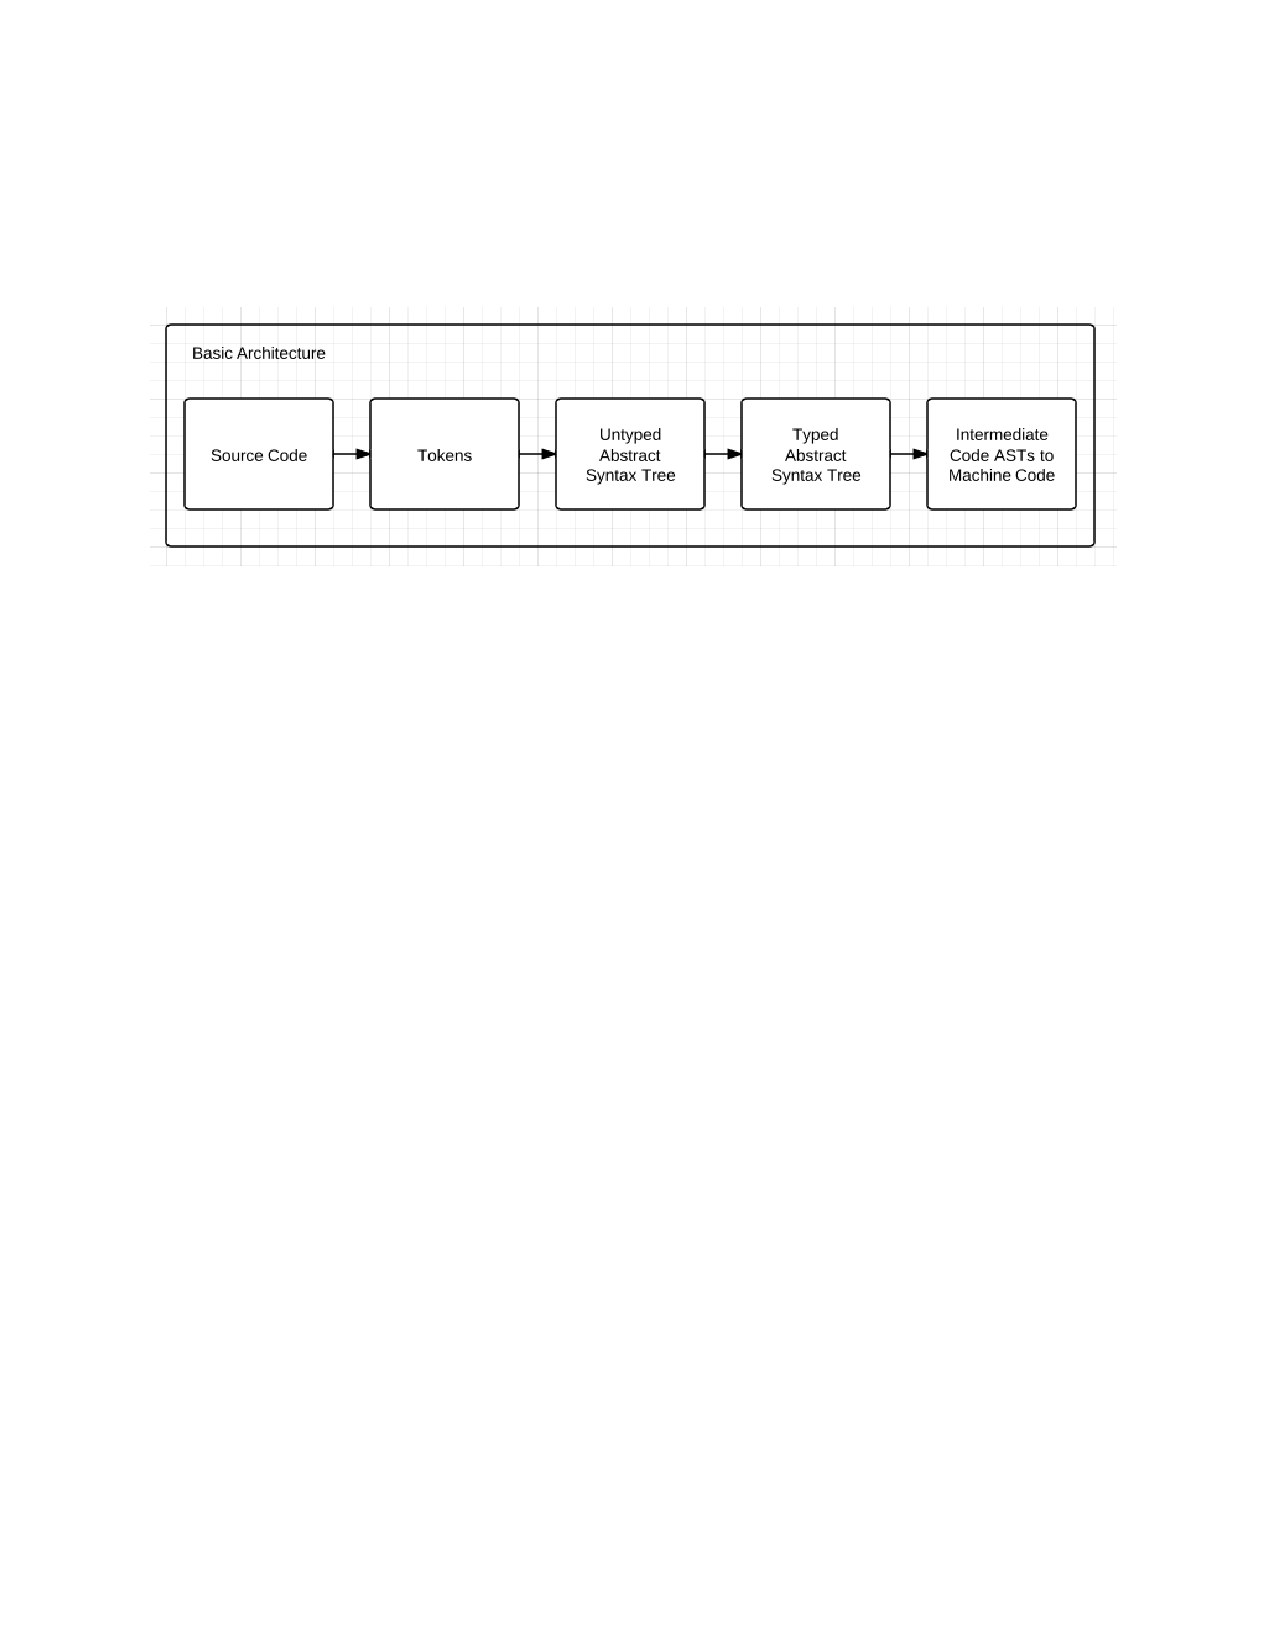
\includegraphics[width=1.0\textwidth]{img/parser_architecture.pdf}
  \caption{The overall architecture of the Hog compilation process.}
\end{figure}
\end{center}

\textbf{@ALL: Do we want to really keep Figure 2?}

Currently, the Hog compiler is implemented as a translator into the Java programming 
language. The first phase of Hog compilation uses the JFlex as its lexical analyzer,
which is designed to work with the Look-Ahead Left-to-Right (LALR) parser generator
CUP. The lexical analyzer creates lexemes, which are logically meaningful sequences,
and for each lexeme the lexlical analyser sends to the LALR parser a token of the
form <token-name, attribute-value>. The second phase of Hog compilation uses Java CUP
to create a syntax tree, which is a tree-like intermediate representation of the source
program, which depics the grammatical structure of the Hog source program.

In the last phase of compilation, the Hog semantic analyzer generates Java source code,
which is then compiled into byte code by the Java compiler. Then with the Hadoop Java Archives
(JARs) the bytecode is executed on the Java Virtual Machine (JVM). With the syntax tree and
the information from the symbol table, the Hog compiler then checks the Hog source program
to ensure semantic consistency with the language specification. The syntax tree is initially
untyped, but after semantic analysis Hog types are added to the syntax tree. Hog types are
represented in two ways, either a translation of a Hog type into a new Java class, or by
mapping Hog types to the equivalent Java types. Mapping Hog types directly to Java types
improves performance because a JVM can handle primitive types much more efficiently than 
objects. Also, a JVM implements optimizations for well-known types, such as String, and 
thus Hog is built for optimal performance.

% section parsing_tools (end)

\section{Linkage and I/O} % (fold)
\label{sec:linkage_and_i_o}

\begin{center}
\begin{figure}
  \label{fig:hog_compiler}
  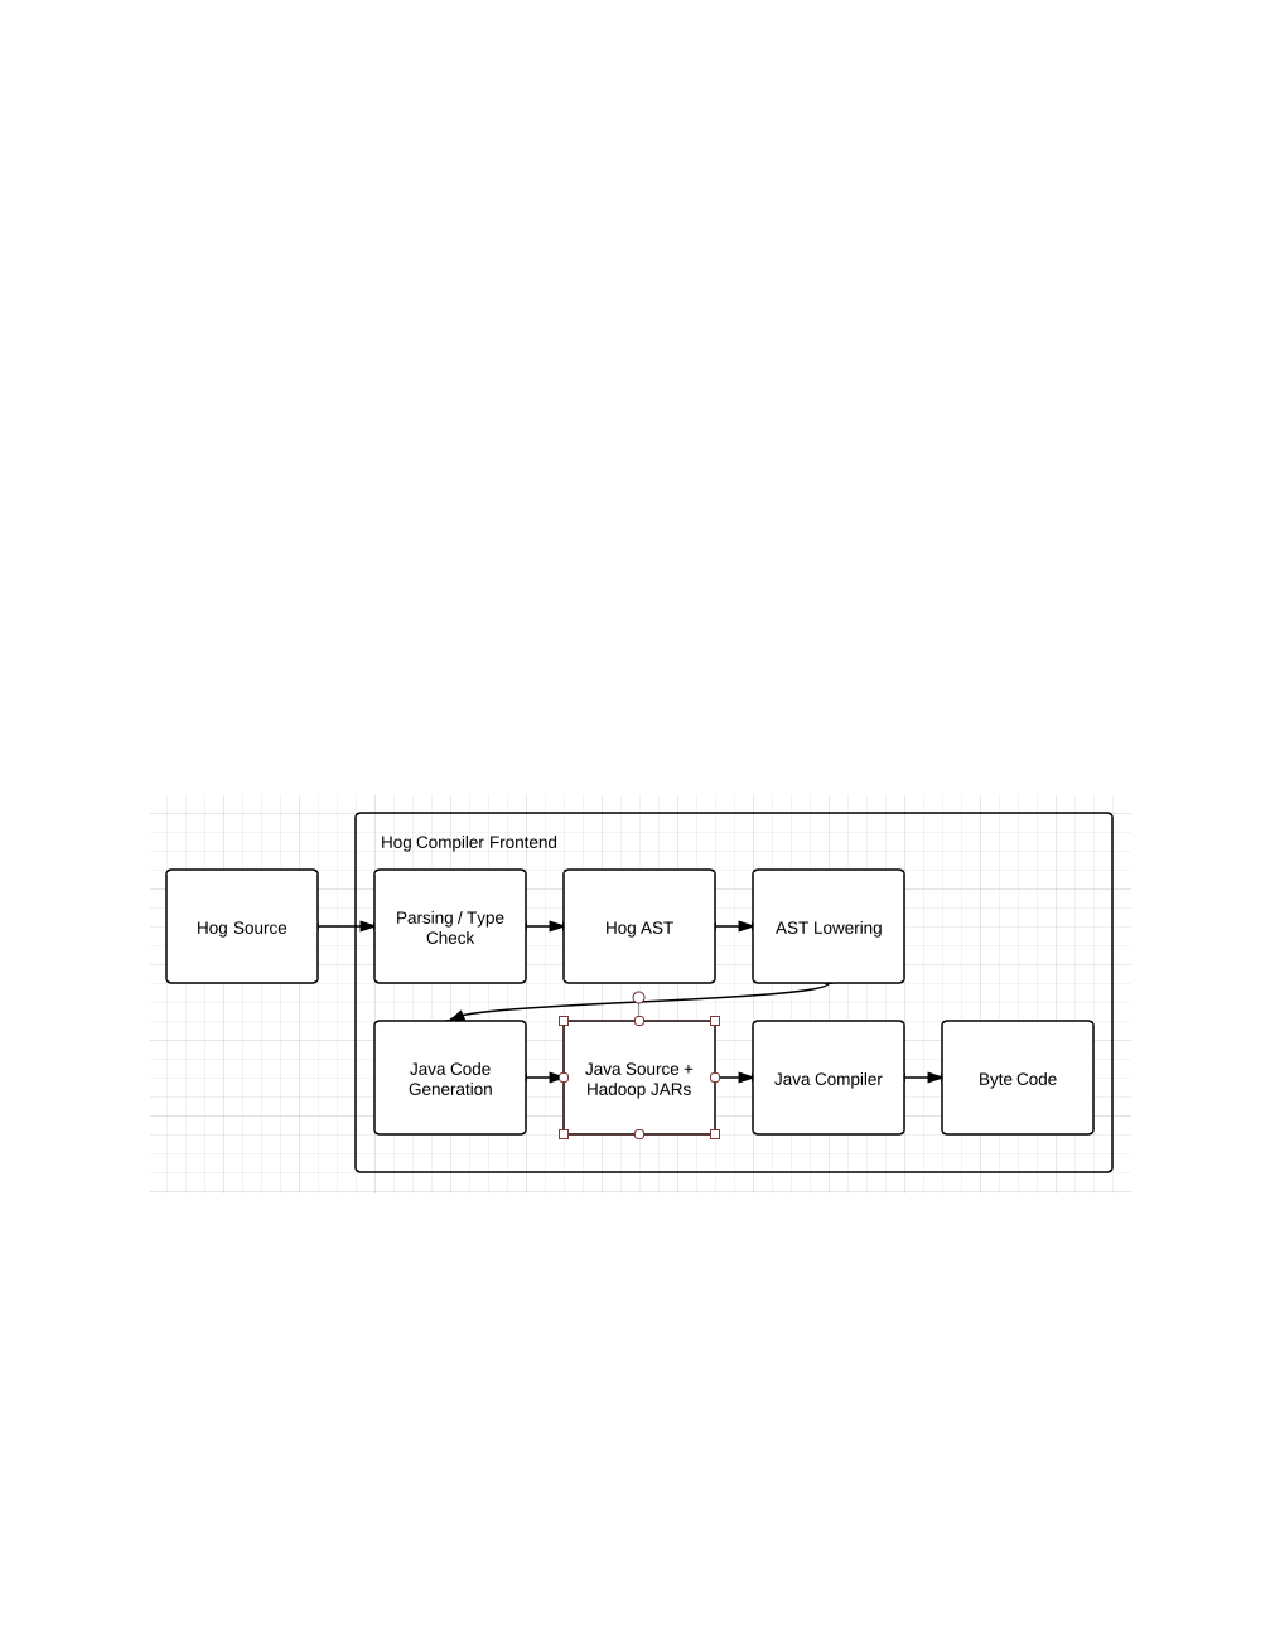
\includegraphics[width=1.0\textwidth]{img/hog_compiler.pdf}
  \caption{The overall structure of the Hog compiler.}
\end{figure}
\end{center}

\subsection{Usage} % (fold)
\label{sub:usage}

% subsection usage (end)

To build and run a Hog source file there is an executable script \tt hog
\rm that automates the compilation and linking steps for the user.

Usage: \tt hog [--hdfs|--local] job <job args> \rm
\begin{itemize}
  \item[] \tt --hdfs\rm: if job ends in '.hog' or '.java' and the file exists, link it against the hadoop JARFILE and then run it on HOST.
  \item[] \tt --local\rm: run on local host.
\end{itemize}

\subsection{Example} % (fold)
\label{sub:example}

\tt hog ­­local WordCountJob.hog ­­input someInputFile.txt ­­output
./someOutputFile.tsv \rm

This runs the \tt wordCount \rm job in \emph{local} mode (i.e. not on a Hadoop
cluster).

% subsection example (end)

% section linkage_and_i_o (end)

\section{Exception Handling} % (fold)
\label{sec:exception_handling}

Similar to other programming languages (Java, C++), Hog uses an exception model in
which an exception is thrown and can be caught by a catch block. Code should be
surrounded by a try block and then any exceptions occurring within the try block
will subsequently be caught by the catch block. Each try block should be
associated with at least one catch block. However, there can be multiple catch
blocks to handle specific types of exceptions. In addition, an optional finally
block can be added. The finally block will execute in all circumstances, whether
or not an exception is thrown. The structure of exception handling should be
similar to this, although there can be multiple catch blocks and the finally block
is optional:

\begin{quotation}
\tt try \{ \rm \\
\indent \indent \emph{expression} \\
\tt \indent \} catch ( \rm \emph{exception} \tt ) \rm \{ \\
\indent \indent \emph{expression} \\
\tt \indent \} finally \rm \{ \\
\indent \indent \emph{expression} \\
\tt \indent \}
\end{quotation}

Because the proper behavior of a Hog program is dependent on resources outside of
the language (i.e. the proper behavior of the user’s Hadoop software), there are
more sources exceptions in Hog than most general purpose languages. These sources
can be divided into three categories: \textbf{\emph{compile­time exceptions}},
\textbf{\emph{internal run­time exceptions}} and \textbf{\emph{external run­time
exceptions}}.

\textbf{@ALL: do we allow exceptions to be thrown? if not we need to say...}

\subsection{Compile-time Exceptions} % (fold)
\label{sub:compile_time_exceptions}

The primary cause of most compile­time exceptions in Hog are syntax errors. Such
errors are unrecoverable because it is impossible for the compiler to properly
interpret the user program. Some compilers for other languages offer a limited
amount of compile­time error correction. Because Hog programs are often designed
to process gigabytes or terabytes of data at a time, the standard Hog compiler
offers no compile­time error correction. The assumption is that a user would
rather re­tool their program than risk the chance of discovering, only after hours
of processing, that the compilers has incorrectly assumed what the user meant. The
following are Hog compile­time exceptions:

\textbf{Add descriptions for each exception}

\textbf{@Jason: fill out decsriptions, make note of the fact that some exceptoins are both run-time and compile-time
(like TypeMismatchException)}

\begin{itemize}
  \item[] \tt IncorrectArgumentException \rm
  
  Thrown when a derived-type object is instantiated with invalid parameters, or a function is called with invalid parameters.
  
  \item[] \tt TypeMismatchException \rm
  
  Thrown when a program attempts to carry out an operation on a variable of the wrong type (like adding a \tt text \rm and an
  \tt int \rm together).
  \item[] \tt ProgramStructureException \rm
  \item[] \tt NoSuchVariableException \rm
  \item[] \tt NoSuchMethodException \rm
  \item[] \tt UnsupportedOperationException \rm
  \item[] \tt RedundantDeclarationException \rm
\end{itemize}

% subsection compile_time_exceptions (end)

\subsection{Internal Run-time Exceptions} % (fold)
\label{sub:internal_run_time_exceptions}

Internal run­time exceptions include such problems as I/O exceptions (i.e. a specified file is not found on either the user’s
local file system or the associated Hadoop file system), type mismatch exceptions (i.e. a program attempts to place two
elements of different types into the same list) and parsing exceptions. The following are Hog internal rum­time exceptions:


\begin{itemize}
  \item[] \tt FileNotFoundException \rm
  
  Thrown when the the Hog program attempts to open a non-existent file.
  
  \item[] \tt FileLoadException \rm
  
  Thrown when an error occurs while Hog is attempting to read a file (e.g. the file is deleted while reading).
  
  \item[] \tt ArrayOutOfBoundsException \rm
  
  Thrown when a program tries to access a non-valid index of a \tt list\rm.
  
  \item[] \tt IncorrectArgumentException \rm
  
  Thrown when a derived-type object is instantiated with invalid parameters, or a function is called with invalid parameters.
  
  \item[] \tt TypeMismatchException \rm
  
  Thrown when a program attempts to carry out an operation on a variable of the wrong type (like adding a \tt text \rm and an
  \tt int \rm together).
  
  \item[] \tt HogMapFunctionException \rm
  
  Thrown when a map function receives a key, value pair of the wrong type.
  
  \item[] \tt HogReduceFunctionException \rm
  
  Thrown when a reduce function receives a key, value pair of the wrong type.
  
  \item[] \tt NullPointerException \rm
  
  Thrown whenever the value of a variable cannot be \tt null \rm (e.g. in \tt myList.get(i)\rm, if \tt i \rm is \tt null\rm,
  the operation with throw a \tt NullPointerException\rm).
  
  \item[] \tt ArithmeticException \rm
  
  Thrown whenever an arithmetic operation is attempted on non-numeric operands.
  
  \item[] \tt IOException \rm
  
  \item[] \tt InterruptedException \rm
  
  \item[] \tt ParseException \rm
\end{itemize}

% section internal_run_time_exceptions (end)

\subsection{External Run-time Exceptions} % (fold)
\label{sub:external_run_time_exceptions}

\textbf{@Kurry, redo this}

% subsection external_run_time_exceptions (end)

% section exception_handling (end)

\section{Grammar} % (fold)
\label{sec:grammar}

\begin{verbatim}


declaration:
   declaration-specifiers

declaration-list:
   declaration
   declaration-list declaration

type-specifier: one of
   void int real bool text


selection-statement:
   if ( expression ) statement
   if ( expression ) statement else statement
   if ( expression ) statement elseif ( expression ) statement... else statement

   switch ( expression ) statement if ( expression ) statement
   if ( expression ) statement else statement
   if ( expression ) statement elseif ( expression ) statement... else statement
 
   switch ( expression ) statement

iteration-statement:  
   while ( expression ) statement
   for ( expression; expression; expression ) statement
   foreach ( expression in array or list) statement

@Functions:
   return­type function­name­1 (parameter­list) {
      exprlist 
   }
   returntype functionname2 (parameterlist){
      exprlist
   }

@Map: 
   (type key­name, type value­name) ­> (type, type) {
      .
      .
      .
  }

unary-operator:
[]

constant:

\end{verbatim}

% section grammar (end)


\end{document}
